\section{Codificação das instruções}
	A codificação das instruções é de fundamental importância para o processamento das operações.	 

	\begin{figure}[H]
    	\centering
    	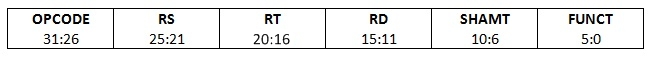
\includegraphics{r-format}
    	\caption{Formato R}
		\label{r_format}
	\end{figure}
  	
	\begin{figure}[H]
    	\centering
    	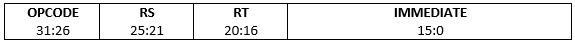
\includegraphics{i-format}
    	\caption{Formato I}
		\label{i_format}
  	\end{figure}
  	
  	\begin{figure}[H]
    	\centering
    	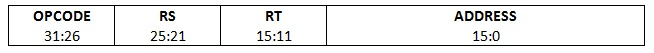
\includegraphics{load-store}
    	\caption{Formato Load/Store}
		\label{loadstore}
  	\end{figure}
  	
   	\begin{figure}[H]
    	\centering
    	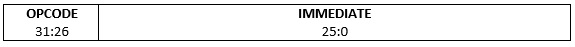
\includegraphics{jump}
    	\caption{Formato Jump}
		\label{jump}
  	\end{figure}
  	
 Todas as instruções contém 32 bits. Exitem 4 formatos de instruções: R, I, Load/Store e Jump. O formato R está relacionado as instruções de 
  	
 